\documentclass{article}

\usepackage{ucs}
\usepackage[utf8]{inputenc}

\usepackage{amsmath, amsfonts, amssymb, amsthm}
\usepackage{fontenc}
\usepackage{graphicx}
\usepackage{mathtools}
\usepackage{tikz}
\usetikzlibrary{calc}
\usepackage{caption}
\usepackage{enumerate}
\usepackage{xcolor}
\usepackage{sectsty}
\usepackage{microtype}
\usepackage[hidelinks]{hyperref}
\usepackage{titlesec}
\usepackage{etoolbox}
\usepackage{enumitem}
\usepackage{chngcntr}

%%%%%%%%%%%%%%%%%%%%%%%%%%%%%%%%%%%%%%%
\newcommand{\spidergraphdistancetwo}[2]{%
    \begin{tikzpicture}[scale=#2] % Scale the entire picture
        \node[draw, circle, thick, inner sep=2pt] at (0,0) (center) {};
        \foreach \n in {1,...,#1}{
            \node[draw, circle, thick, inner sep=2pt] at ({\n*360/#1}:0.3cm) (n\n) {};
            \draw[thick] (center)--(n\n);
            \node[draw, circle, thick, inner sep=2pt] at ({\n*360/#1}:0.6cm) (m\n) {}; % New nodes at twice the distance
            \draw[thick] (n\n)--(m\n); % Connect the new nodes
        }
    \end{tikzpicture}%
}

\newcommand{\spidergraphdistancethree}[2]{%
    \begin{tikzpicture}[scale=#2] % Scale the entire picture
        \node[draw, circle, thick, inner sep=2pt] at (0,0) (center) {};
        \foreach \n in {1,...,#1}{
            \foreach \i in {1,2,3}{
                \node[draw, circle, thick, inner sep=2pt] at ({\n*360/#1}:\i*0.3cm) (n\n\i) {};
                \ifnum\i=1
                    \draw[thick] (center)--(n\n\i);
                \else
                    \draw[thick] (n\n\the\numexpr\i-1\relax)--(n\n\i);
                \fi
            }
        }
    \end{tikzpicture}%
}
%%%%%%%%%%%%%%%%%%%%%%%%%%%%%%%%%%%%%%%

% Define the exercise environment with section-dependent numbering
\theoremstyle{definition}
\newtheorem{exercise}{Exercise}[section]

% Redefine the numbering format to show only the exercise number within the section
\renewcommand{\theexercise}{\arabic{exercise}}

% Keep the existing numbering scheme for other environments
\theoremstyle{definition}
\newtheorem{defn}{Definition}[section]
\newtheorem{question}{Question}[section]
\newtheorem{example}{Example}[section]
\newtheorem{problem}{Problem}[section]
\newtheorem{notation}{Notation}
\newtheorem{challenge}[exercise]{Challenge}

% Use a separate counter for theorems, lemmas, corollaries, propositions, and conjectures
\newtheorem{theorem}{Theorem}
\newtheorem{proposition}[theorem]{Proposition}
\newtheorem{lemma}[theorem]{Lemma}
\newtheorem{corollary}[theorem]{Corollary}
\newtheorem{conjecture}{Conjecture}

\newenvironment{solution}{\noindent\emph{Solution.}}{\hfill$\square$}

\theoremstyle{remark}
\newtheorem*{remark}{Remark}

%%%%%%%%%%%%%%%%%%%%%%%%%%%%%%%%%%%%%%%

\newcommand{\R}{\mathbb{R}}
\newcommand{\C}{\mathbb{C}}
\newcommand{\Z}{\mathbb{Z}}
\newcommand{\Q}{\mathbb{Q}}
\newcommand{\N}{\mathbb{N}}
\newcommand{\calP}{\mathcal{P}}
\newcommand{\powerset}[1]{\mathscr{P}(#1)}

%%%%%%%%%%%%%%%%%%%%%%%%%%%%%%%%%%%%%%%

\title{Asymmetric Colorings of Graphs}
\author{Ata Berk Saraç}
\date{Summer 2024}

\begin{document}
\maketitle

% Define colors
\definecolor{sectioncolor}{RGB}{0, 102, 204}
\definecolor{subsectioncolor}{RGB}{211, 65, 63}
\definecolor{othercolor}{RGB}{0, 128, 0}

% Apply the color to section titles
\sectionfont{\color{sectioncolor}}
\subsectionfont{\color{subsectioncolor}}

%%%%%%%%%%%%%%%%%%%%%%%%%%%%%%%%%%%%%%%

 \section{First Week}

%%%%%%%%%%%%%%%%%%%%%%%%%%%%%%%%%%%%%%%
 \subsection{Preliminaries}

 \begin{defn}
     A \textit{graph} $G$ is a pair of sets, $G=(V,E)$ such that $V$ (or $V(G)$ to underline that this set is related to $G$) is a nonempty set called a \textit{vertex-set} and $E\subseteq \binom{V}{2}$ (or $E(G)$) is called an \textit{edge-set}, elements of $V$ are called \textit{vertices} and elements of $E$ are called \textit{edges}. An edge consisting of vertices $u$ and $v$ will be denoted as $uv$.
 \end{defn}
%%%%%
 \begin{defn}
    An \textit{automorphism} of a graph $G=(V,E)$ is a bijection $\phi:V\to V$ such that $uv\in E$ if and only if $\phi(u)\phi(v)\in E$, for any pair of vertices $u$ and $v$.

    An \textit{edge automorphism} of $G$ is a bijection $\sigma : E \to E$ such that edges $x$ and $y$ are incident if and only if $\sigma (x)$ and $\sigma (y)$ are incident.
 \end{defn}

\begin{remark}
 Every graph admits the identity, or trivial, automorphism which maps every vertex to itself.
\end{remark}
%%%%%
\begin{defn}
    A \textit{vertex fixing set} of a graph $G$, denoted $f(G)$, is a subset $X\subseteq V(G)$ for which the only automorphism of $G$ that fixes $X$ point-wise is the trivial automorphism. I.e., if $f(x)=x$ for all $x\in X$, then $f(v)=v$ for all $v\in V$. The \textit{vertex fixing number} of $G$ is the minimum cardinality of a vertex fixing set of $G$.

    Analogously, an \textit{edge fixing set} of a graph $G$, denoted $f'(G)$, is a subset $X\subseteq E(G)$ for which the only automorphism of $G$ that fixes $X$ point-wise is the trivial automorphism. I.e., if $f(x)=x$ for all $x\in X$, then $f(e)=e$ for all $e\in E$. The \textit{edge fixing number} of $G$ is the minimum cardinality of an edge fixing set of $G$.
\end{defn}

\begin{defn}
    A \textit{vertex coloring} of a graph $G=(V,E)$ is a function $c:V\to \N$ that assigns a natural number (or color) to each vertex of $G$. An \textit{asymmetric vertex coloring} of $G$ is a vertex coloring such that the only automorphism of $G$ that preserves the color classes is the trivial automorphism. The \textit{asymmetric vertex coloring number} of $G$, denoted $a(G)$, is the minimum number of colors required to asymmetrically color the vertices of $G$.

    Analogously, an \textit{edge coloring} of a graph $G=(V,E)$ is a function $c:E\to \N$ that assigns a natural number (or color) to each edge of $G$. An \textit{asymmetric edge coloring} of $G$ is an edge coloring such that the only automorphism of $G$ that preserves the color classes is the trivial automorphism. The \textit{asymmetric edge coloring number} of $G$, denoted $a'(G)$, is the minimum number of colors required to asymmetrically color the edges of $G$.
\end{defn}

\begin{defn}
    In a graph $G$, two vertices $u$ and $v$ are called \textit{connected} if $G$ contains a path from $u$ to $v$. Otherwise, they are called \textit{disconnected}. If the two vertices are additionally connected by a path of length $1$ (that is, they are the endpoints of a single edge), the vertices are called \textit{adjacent}.
    
    A graph is said to be \textit{connected} if every pair of vertices in the graph is connected. This means that there is a path between every pair of vertices. A graph that is not connected is called \textit{disconnected}. A graph $G$ is therefore disconnected if there exist two vertices in $G$ such that no path in $G$ has these vertices as endpoints. E.g., a graph with just one vertex is connected, an edgeless graph with two or more vertices is disconnected.
\end{defn}

\begin{defn}
    Given a graph $G$, its \textit{line graph} $L(G)$ is a graph such that each vertex of $L(G)$ represents an edge of $G$; and two vertices of $L(G)$ are adjacent if and only if their corresponding edges share a common endpoint (in other words, they are incident) in $G$.
\end{defn}
%%%%%
 \begin{defn}
 A \textit{cycle graph} $C_n$ is a graph associated to a polygon with $n$ vertices. That is, the vertices of $C_n$ can be placed around a circle so that two vertices are adjacent if and only if they appear consecutively along the circle.
 \end{defn}
%%%%%
 \begin{defn}
 A \textit{path graph}, denoted $P_n$, is a graph whose vertices can be listed in the order $v_1, v_2,\ldots, v_{n+1}$ such that the edges are $\{v_i, v_{i+1}\}$ where $i = 1, 2,\ldots, n$. Equivalently, a \textit{path} with at least two vertices is connected and has two \textit{terminal vertices} (vertices that have degree 1), while all other vertices (if any) have degree 2.
 \end{defn}
%%%%%
 \begin{defn}
 The \textit{complete graph} on $n$ vertices, denoted $K_n$, is the graph for which every pair of vertices has a connecting edge.
 \end{defn}
%%%%%
 \begin{defn}
 A \textit{star graph} on $n+1$ vertices, denoted $S_n$, is a graph consisting of a single vertex (we call it \textit{central vertex}) connected to $n$ other vertices.
 \end{defn}

\begin{defn}
The \textit{distance} between two vertices in a graph $G$ is the number of edges in a shortest path connecting them. We denote it by $d\{v_i,v_j\}$ for all $v_i, v_j \in G$. Note that $d\{v_i,v_j\}=d\{v_j,v_i\}$.
\end{defn}

\begin{defn}
    The \textit{degree} of a vertex, denoted $\delta(v)$ in a graph is the number of edges incident to it.
\end{defn}

\begin{notation}
Let $v$ be a vertex of a graph $G$, and let $c(v)=i$, where $i \in \N$. We denote \textit{color classes} by $\overline{i}$. Note that $\overline{i} = \overline{j}$ if and only if $i = j$.
\end{notation}

%%%%%%%%%%%%%%%%%%%%%%%%%%%%%%%%%%%%%%%

 \subsection{Exercises}
%%%%%
 
 \begin{exercise}\label{ex1.1}
 Find the minimum number of colors required to break the symmetries of $C_4$, and $C_5$.
 \end{exercise}
 
 \begin{solution}
 We know that $a(C_n) \neq 1$ for all $n \ge 2$. 
 
 Say $a(C_4)=2$, then either
 
 \begin{enumerate}[label=\roman*.]
    \item three vertices have the same color (one of them must be adjacent to the other two) and one vertex has a different color. But we see that two non-adjacent vertices with the same color can be mapped to one another;
 
    \item two vertices have the same color (either adjacent or non-adjacent) and two vertices have a different color. But if two adjacent vertices have the same color, they can be mapped onto each other, and the remaining vertices with different colors can also be mapped onto each other. If they are non-adjacent similar mappings exist. 
 \end{enumerate}
 
 Whereas if $a(C_4)=3$ and we color two vertices with the color $i$, and color the remaining vertices with two colors distinct to each other and to $i$, then the only automorphism left is the trivial automorphism. Since no two vertices can have adjacent vertices with the same pair of color classes.

 For $C_5$, by a similar process of trial-and-error, we find that $a(C_5)=3$.

 As a side note, by the upcoming Theorem \ref{thm1}, $a'(C_n)=L(a(C_n))$ since $C_n$ and the line graph $L(C_n)$ are isomorphic for all $n \ge 3$.
 \end{solution}
%%%%%
 \begin{exercise}\label{ex1.2}
 Determine this value for $C_n$ when $n \ge 6$.
 \end{exercise}
 
 \begin{solution}
 Our solution does not equal $1$ since cycle graphs are symmetric. We claim that the answer is $2$, to that end, choose a random vertex $v \in C_n$ and color it with the natural number $1$, we follow the process below:

\begin{enumerate}[label=\roman*.]
 \item If $n$ is an even number, then find the vertex with distance $n/2$ to $v$ and color one with $2$. If $n$ is an odd number, then find the vertex with distance $\lfloor n/2 \rfloor$ to $v$ and color a random one with $2$. Independent of whether $n$ is even or not, call this vertex $v_1$.
 
 \item Let $u_1$ and $u_2$ be the vertices that has distance $1$ to $v_1$. Color $u_1$ with $1$ and $u_2$ with $2$.

 \item Finally, find the vertices that has distance $\lfloor n/3 \rfloor$ and color the one that has a greater distance to $u_2$ with $2$. Call this vertex $v_2$.

 \item Color the rest of the vertices with $1$.
 \end{enumerate}

 This process breaks the symmetries of $C_n$ for $n\ge 6$ since the distance of each vertex that we colored with $1$ has different distances to each of the three vertices $v_1$, $v_2$, and $u_2$.
 
 Hence, we find that $a(C_n)=2$ whenever $n \ge 6$ as predicted.
 \end{solution}
%%%%%
 \begin{exercise}
 Find the asymmetric vertex coloring number of $P_5$.
 \end{exercise}
 
 \begin{solution}
 We see that if one of the terminal points (say $v_1$) has a different color class than all of the remaining vertices, then we shall be done. This is because $d\{v_1,v_i\} \neq d\{v_1,v_j\}$ for two distinct vertices $v_i,v_j \in P_5$, and so there cannot exist any automorphism, except the trivial automorphism. Thus, the answer is $2$.
 
 This is only one of the solutions, but other solutions are quite similar, and the terminal points are easier to observe and explain. Additionally, we find, by the upcoming Theorem \ref{thm1} that $a'(P_5)=2$ as well.
 \end{solution}
%%%%%
 \begin{exercise}
 Determine the asymmetric vertex coloring numbers for paths $P_n$ of any length.
 \end{exercise}

 \begin{solution}
 We determine that $a(P_n)=2$ for paths $P_n$ of any length. The logic in the previous exercise applies to this one as well.
 \end{solution}
%%%%%
 \begin{exercise}\label{ex1.5}
 Find the asymmetric vertex coloring number of $K_n$.
 \end{exercise}
 
 \begin{solution}
 We find that $a(K_n)=n$ for any $n \in \N$. If $a(K_n)$ was less than $n$, it would follow, by the definition of $K_n$, that there exists an automorphism $\phi$ such that $\phi(v_i)=v_j$ for some distinct $v_i,v_j \in V(K_n)$ (exclude $K_1$ because it is trivial).
 \end{solution}
%%%%%
 \begin{exercise}\label{ex1.6}
 Find the asymmetric edge coloring number of $K_n$.
 \end{exercise}
 
 \begin{solution}
 We find that $a'(K_1)=0$, $a'(K_2)=1$ , and $a'(K_3)=a'(K_4)=a'(K_5)=3$. For $K_n$, where $n \ge 6$ we run a near-identical process to Exercise \ref{ex1.2}. Hence, we find that $a'(K_n)=2$ for all $n \ge 6$.
 \end{solution}
%%%%%
 \begin{exercise}
 Find the asymmetric vertex and edge coloring numbers of the star $S_n$, for any $n \ge 2$.
 \end{exercise}
 
 \begin{solution}
 We find that $a(S_n)=a'(S_n)=n$ for all $n \in \N$. Say two distinct vertices $v_i, v_j \in V(S_n)$ of degree $1$ have the same colors, then since all vertices are incident to one and the same vertex and no other vertex, we can find an automorphism $\phi$ so that $\phi(v_i)=v_j$. A similar approach can be followed to find the asymmetric edge coloring number of $S_n$ for any $n \ge 2$.
 \end{solution}
%%%%%
 \begin{exercise}
 Find the fixing number of the star $S_n$, for any $n \ge 2$.
 \end{exercise}
 
 \begin{solution}
 If $f(S_n) < n-1$, then two non-central vertices can be mapped to one another. Thus, we find that $f(S_n)=n-1$ (and not $n$ since either way no two vertices could be mapped to one another).
 \end{solution}
%%%%%
 \begin{exercise}
 Can you determine a general relationship between the asymmetric vertex coloring number and the fixing number of a graph?
 \end{exercise}
 
 \begin{solution}
 Let $G$ be a non-empty graph. Color each fixed vertex of a graph with distinct natural numbers (say $i$, where $i=1,\ldots,f(G)$), i.e., each fixed vertex has a distinct color class $\overline{i}$ and each non-fixed vertex is colored by a single number --but not any of the previous natural numbers $i$. This should guarantee us to obtain an asymmetric graph. By this explanation, $a(G)$ cannot be greater than $f(G)+1$ but it can be equal to it. Thus, we have the inequality $a(G) \le f(G)+1$.
 
 As a further observation, coloring each vertex by some $i$ serves as fixing that vertex because the vertex with the color class $\overline{i}$ cannot be mapped to any vertex that has a distinct color class $\overline{j}$.
 \end{solution}
%%%%%
 \begin{exercise}
 Find asymmetric vertex colorings of the following two graphs using only two colors (say, red and blue). Determine their fixing numbers too.

%%%%%%%%%%%%%%%%%%%%%%%%%%%%%%%%%%%%%%%%
\begin{center}
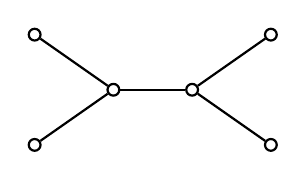
\begin{tikzpicture}
  % Nodes
  \node[draw, circle, thick, inner sep=1.5pt] (a) at (2, 0) {};
  \node[draw, circle, thick, inner sep=1.5pt] (b) at (1, 0.7) {};
  \node[draw, circle, thick, inner sep=1.5pt] (c) at (1, -0.7) {};
  \node[draw, circle, thick, inner sep=1.5pt] (d) at (4, 0.7) {};
  \node[draw, circle, thick, inner sep=1.5pt] (e) at (4, -0.7) {};
  \node[draw, circle, thick, inner sep=1.5pt] (f) at (3, 0) {};

  % Edges
  \draw[thick] (a) -- (f);
  \draw[thick] (a) -- (b);
  \draw[thick] (a) -- (c);
  \draw[thick] (d) -- (f);
  \draw[thick] (e) -- (f);
\end{tikzpicture}
\hspace{1cm} %%%%%%%%%%%%%%%%%%%%%%%%%%%%%%%%%%%%%%%
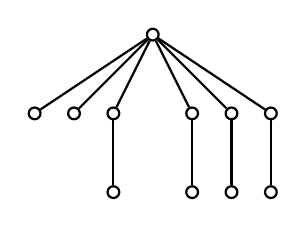
\begin{tikzpicture}
  % Nodes
 \node[draw, circle, thick, inner sep=1.5pt] (a) at (0, 2) {};
  \node[draw, circle, thick, inner sep=1.5pt] (b) at (-1.5, 1) {};
  \node[draw, circle, thick, inner sep=1.5pt] (c) at (-1, 1) {};
  \node[draw, circle, thick, inner sep=1.5pt] (d) at (-0.5, 1) {};
  \node[draw, circle, thick, inner sep=1.5pt] (e) at (0.5, 1) {};
  \node[draw, circle, thick, inner sep=1.5pt] (f) at (1, 1) {};
  \node[draw, circle, thick, inner sep=1.5pt] (g) at (1.5, 1) {};
  
  \node[draw, circle, thick, inner sep=1.5pt] (h) at (-0.5, 0) {};
  \node[draw, circle, thick, inner sep=1.5pt] (i) at (0.5, 0) {};
  \node[draw, circle, thick, inner sep=1.5pt] (j) at (1, 0) {};
  \node[draw, circle, thick, inner sep=1.5pt] (k) at (1.5, 0) {};
  
  % Edges
  \draw[thick] (a) -- (b);
  \draw[thick] (a) -- (c);
  \draw[thick] (a) -- (d);
  \draw[thick] (a) -- (e);
  \draw[thick] (a) -- (f);
  \draw[thick] (a) -- (g);

  \draw[thick] (d) -- (h);
  \draw[thick] (e) -- (i);
  \draw[thick] (f) -- (j);
  \draw[thick] (g) -- (k);
\end{tikzpicture}
\end{center} 
%%%%%%%%%%%%%%%%%%%%%%%%%%%%%%%%%%%%%%%
 \end{exercise}
 
 \begin{solution}
 Let the graphs above be graphs $G$ (graph to the left) and $H$ (graph to the right). It follows by trial-and-error that $a(G)$ and $a(H)$ equal $2$. A solution for each graph are drawn below:
 
%%%%%%%%%%%%%%%%%%%%%%%%%%%%%%%%%%%%%%%%
\begin{center}
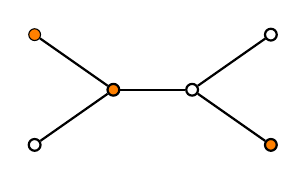
\begin{tikzpicture}

  \node[draw, fill=orange, circle, thick, inner sep=1.5pt] (a) at (2, 0) {};
  \node[draw, fill=orange, circle, inner sep=1.5pt] (b) at (1, 0.7) {};
  \node[draw, circle, thick, inner sep=1.5pt] (c) at (1, -0.7) {};
  \node[draw, circle, thick, inner sep=1.5pt] (d) at (4, 0.7) {};
  \node[draw, fill=orange, circle, thick, inner sep=1.5pt] (e) at (4, -0.7) {};
  \node[draw, circle, thick, inner sep=1.5pt] (f) at (3, 0) {};

  \draw[thick] (a) -- (f);
  \draw[thick] (a) -- (b);
  \draw[thick] (a) -- (c);
  \draw[thick] (d) -- (f);
  \draw[thick] (e) -- (f);
\end{tikzpicture}
\hspace{1cm} %%%%%%%%%%%%%%%%%%%%%%%%%%%%%%%%%%%%%%%
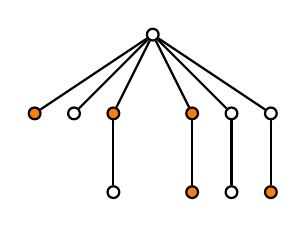
\begin{tikzpicture}
  % Nodes
 \node[draw, circle, thick, inner sep=1.5pt] (a) at (0, 2) {};
  \node[draw, fill=orange, circle, thick, inner sep=1.5pt] (b) at (-1.5, 1) {};
  \node[draw, circle, thick, inner sep=1.5pt] (c) at (-1, 1) {};
  \node[draw, fill=orange, circle, thick, inner sep=1.5pt] (d) at (-0.5, 1) {};
  \node[draw, fill=orange, circle, thick, inner sep=1.5pt] (e) at (0.5, 1) {};
  \node[draw, circle, thick, inner sep=1.5pt] (f) at (1, 1) {};
  \node[draw, circle, thick, inner sep=1.5pt] (g) at (1.5, 1) {};
  
  \node[draw, circle, thick, inner sep=1.5pt] (h) at (-0.5, 0) {};
  \node[draw, fill=orange, circle, thick, inner sep=1.5pt] (i) at (0.5, 0) {};
  \node[draw, circle, thick, inner sep=1.5pt] (j) at (1, 0) {};
  \node[draw, fill=orange, circle, thick, inner sep=1.5pt] (k) at (1.5, 0) {};

  \draw[thick] (a) -- (b);
  \draw[thick] (a) -- (c);
  \draw[thick] (a) -- (d);
  \draw[thick] (a) -- (e);
  \draw[thick] (a) -- (f);
  \draw[thick] (a) -- (g);

  \draw[thick] (d) -- (h);
  \draw[thick] (e) -- (i);
  \draw[thick] (f) -- (j);
  \draw[thick] (g) -- (k);
\end{tikzpicture}
\end{center}
 \end{solution}
%%%%%
 \begin{exercise}
Given the set of automorphisms of a graph $G$, can you determine the fixing number of $G$?

 \end{exercise}
 
 \begin{solution}
 No, one cannot determine the fixing number of a graph $G$ given the set of automorphisms of $G$.

 This requires an explanation.
 \end{solution}

%%%%%%%%%%%%%%%%%%%%%%%%%%%%%%%%%%%%%%%

 \section{Second Week}

%%%%%%%%%%%%%%%%%%%%%%%%%%%%%%%%%%%%%%%
 \subsection{Preliminaries}
%%%%%%%%%%%%%%%%%%%%%%%%%%%%%%%%%%%%%%%
 \begin{defn}
 A \textit{caterpillar} is a graph that consists of a path and a set of \textit{feet}, which are vertices connected directly to the path by an edge. I.e., a caterpillar or \textit{caterpillar tree} is a tree in which all the vertices are within distance 1 of a central path.
 \end{defn}
%%%%%
 \begin{defn}
 A \textit{spider} is a graph that consists of disjoint paths and a vertex which is connected by an edge to a terminal vertex on each path.
 \end{defn}
%%%%%
 \begin{defn}
 For a graph $G = (V,E)$, the \textit{line graph} of $G$, denoted $L(G)$, is the graph whose vertices are the elements of $E$ and whose edges join pairs $e$, $f \in E$ which are incident in $G$ (share a common endpoint).
 \end{defn}
%%%%%

 \begin{theorem}\label{thm1}
 Let $G$ be a connected graph which is neither a single edge nor $K_{4} - e$. Then $a'(G) = a(L(G))$.
 \end{theorem}

 \begin{proof}
 I know the proof, will write it down later.
 \end{proof}
 
%%%%%

 \begin{defn}
 Let $G_1 = (V_1, E_1)$ and $G_2 = (V_2, E_2)$ be graphs. The Kronecker product of $G_1$ and $G_2$, which we will denote by $G_1 \otimes G_2$, is the graph on the vertex-set $V_1 \times V_2 := \{(v_1,v_2) : v_1 \in V_1,v_2 \in V_2)\}$ and where there is an edge between the vertices $(v_1, v_2)$ and $(v'_1 , v'_2)$ if and only if there are edges $\{v_1, v'_1 \} \in E_1 $and $\{v_2, v'_2\} \in E_2$.
 \end{defn}

 \begin{defn}
 Let $G$ be a graph with vertex-set $V$ and edge-set $E$. An edge automorphism of $G$ is a bijection $\sigma: E \to E$ such that edges $x$ and $y$ are incident if and only if $\sigma(x)$ and $\sigma(y)$ are incident.
 \end{defn}

 \begin{defn}
 Let an edge fixing set of a graph $G$ is a subset $Y \subseteq E$ for which the only automorphism of $G$ that fixes $Y$ pointwise is the trivial automorphism. The edge fixing number of $G$, denoted $f'(G)$, is the minimum cardinality of an edge fixing set of $G$.
 \end{defn}

 \begin{defn}
 The wheel graph on $n + 1$ vertices, denoted $W_{n+1}$ is the cycle of length $n$ with an additional vertex connected to all other vertices.
 \end{defn}
 
%%%%%%%%%%%%%%%%%%%%%%%%%%%%%%%%%%%%%%%

 \subsection{Exercises}
%%%%%
 \begin{exercise}
 Find the asymmetric vertex coloring numbers of the following graphs:
 
\begin{center}
 \vspace{0.3cm}
 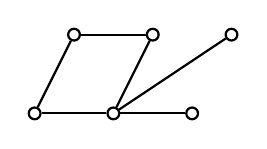
\begin{tikzpicture}
    \node[draw, circle, thick, inner sep=1.5pt] (a) at (0, 0) {};
    \node[draw, circle, thick, inner sep=1.5pt] (b) at (1, 0) {};
    \node[draw, circle, thick, inner sep=1.5pt] (c) at (2, 0) {};
    \node[draw, circle, thick, inner sep=1.5pt] (d) at (0.5, 1) {};
    \node[draw, circle, thick, inner sep=1.5pt] (e) at (1.5, 1) {};
    \node[draw, circle, thick, inner sep=1.5pt] (f) at (2.5, 1) {};

    \draw[thick] (a) -- (b);
    \draw[thick] (a) -- (d);
    \draw[thick] (b) -- (a);
    \draw[thick] (b) -- (c);
    \draw[thick] (b) -- (f);
    \draw[thick] (d) -- (e);
    \draw[thick] (b) -- (e);
\end{tikzpicture}
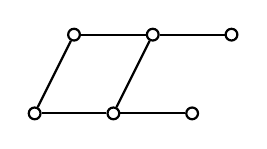
\begin{tikzpicture}
    \node[draw, circle, thick, inner sep=1.5pt] (a) at (0, 0) {};
    \node[draw, circle, thick, inner sep=1.5pt] (b) at (1, 0) {};
    \node[draw, circle, thick, inner sep=1.5pt] (c) at (2, 0) {};
    \node[draw, circle, thick, inner sep=1.5pt] (d) at (0.5, 1) {};
    \node[draw, circle, thick, inner sep=1.5pt] (e) at (1.5, 1) {};
    \node[draw, circle, thick, inner sep=1.5pt] (f) at (2.5, 1) {};

    \draw[thick] (a) -- (b);
    \draw[thick] (a) -- (d);
    \draw[thick] (b) -- (a);
    \draw[thick] (b) -- (c);
    \draw[thick] (d) -- (e);
    \draw[thick] (b) -- (e);
    \draw[thick] (e) -- (f);
\end{tikzpicture}
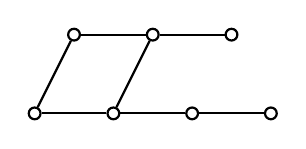
\begin{tikzpicture}
    \node[draw, circle, thick, inner sep=1.5pt] (a) at (0, 0) {};
    \node[draw, circle, thick, inner sep=1.5pt] (b) at (1, 0) {};
    \node[draw, circle, thick, inner sep=1.5pt] (c) at (2, 0) {};
    \node[draw, circle, thick, inner sep=1.5pt] (c') at (3, 0) {};
    \node[draw, circle, thick, inner sep=1.5pt] (d) at (0.5, 1) {};
    \node[draw, circle, thick, inner sep=1.5pt] (e) at (1.5, 1) {};
    \node[draw, circle, thick, inner sep=1.5pt] (f) at (2.5, 1) {};

    \draw[thick] (a) -- (b);
    \draw[thick] (a) -- (d);
    \draw[thick] (b) -- (a);
    \draw[thick] (b) -- (c);
    \draw[thick] (d) -- (e);
    \draw[thick] (b) -- (e);
    \draw[thick] (e) -- (f);
    \draw[thick] (c) -- (c');
\end{tikzpicture}
\vspace{0.3cm}
\end{center}

 \noindent For each graph above, find the maximum number of vertices colored 1 in an asymmetric vertex coloring using a minimum number of colors.
 \end{exercise}
 
 \begin{solution}
 Let $G$, $H$, and $I$ be the name of the graphs from left to right. We find that $a(G)=1$, $a(H)=2$, and $a(I)=1$.
 \end{solution}

 \begin{exercise}
 Can you find the asymmetric coloring number of the following caterpillar? Are there ways to generalize this to other caterpillars?

\begin{center}
\vspace{0.3cm}
 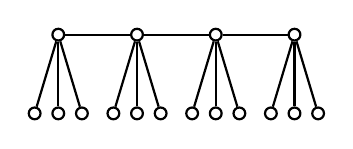
\begin{tikzpicture}
    \node[draw, circle, thick, inner sep=1.5pt] (a) at (0, 1) {};
    \node[draw, circle, thick, inner sep=1.5pt] (b) at (1, 1) {};
    \node[draw, circle, thick, inner sep=1.5pt] (c) at (2, 1) {};
    \node[draw, circle, thick, inner sep=1.5pt] (d) at (3, 1) {};
    
    \node[draw, circle, thick, inner sep=1.5pt] (a1) at (-0.3, 0) {};
    \node[draw, circle, thick, inner sep=1.5pt] (a2) at (0, 0) {};
    \node[draw, circle, thick, inner sep=1.5pt] (a3) at (0.3, 0) {};

    \node[draw, circle, thick, inner sep=1.5pt] (b1) at (0.7, 0) {};
    \node[draw, circle, thick, inner sep=1.5pt] (b2) at (1, 0) {};
    \node[draw, circle, thick, inner sep=1.5pt] (b3) at (1.3, 0) {};

    \node[draw, circle, thick, inner sep=1.5pt] (c1) at (1.7, 0) {};
    \node[draw, circle, thick, inner sep=1.5pt] (c2) at (2, 0) {};
    \node[draw, circle, thick, inner sep=1.5pt] (c3) at (2.3, 0) {};

    \node[draw, circle, thick, inner sep=1.5pt] (d1) at (2.7, 0) {};
    \node[draw, circle, thick, inner sep=1.5pt] (d2) at (3, 0) {};
    \node[draw, circle, thick, inner sep=1.5pt] (d3) at (3.3, 0) {};

  \draw[thick] (a) -- (b);
  \draw[thick] (b) -- (c);
  \draw[thick] (c) -- (d);
  
  \draw[thick] (a) -- (a1);
  \draw[thick] (a) -- (a2);
  \draw[thick] (a) -- (a3);

  \draw[thick] (b) -- (b1);
  \draw[thick] (b) -- (b2);
  \draw[thick] (b) -- (b3);
  
  \draw[thick] (c) -- (c1);
  \draw[thick] (c) -- (c2);
  \draw[thick] (c) -- (c3);

  \draw[thick] (d) -- (d1);
  \draw[thick] (d) -- (d2);
  \draw[thick] (d) -- (d3);
 \end{tikzpicture}
 \end{center}
 
 \end{exercise}

 \begin{solution}
 Observe that the vertices on the path are not important, the important vertices are the feet. The caterpillar above has the asymmetric coloring number $3$ since if any of the two feet were to be in the same color class, then they could be mapped onto each other, which would be an automorphism other than identity.

 Let $C$ be a caterpillar. Since each foot of $C$ must have a different color and there exists a vertex (or vertices) $v$ of $C$ such that $v$ has the highest number of (say $n$) feet compared to other vertices on the path (i.e., vertices with the same distance to a vertex $v$), then $n$ has to be the asymmetric coloring number of $C$.
 \end{solution}

 \begin{exercise}
 Can you find the asymmetric coloring numbers of the following two gorgeous spiders that took a lot of time to draw? Can you generalize this to other spiders whose “legs” have the same numbers of vertices?
    \begin{center}
        \spidergraphdistancetwo{5}{2}
        \hspace{0.3cm}
        \spidergraphdistancethree{5}{2}
    \end{center}
 \end{exercise}

 \begin{solution}
 For the spider to the left it is $3$, to see this first observe that central vertex
 \end{solution}
%%%%%
 \begin{exercise}
 In the exercises of Week 1, we saw that all path graphs on $n \ge 2$ vertices have asymmetric coloring number $2$. This gives us an infinite family of graphs with asymmetric coloring number $2$. Cycles on $n \ge 6$ vertices are another example of such an infinite family. Can you give an example of an infinite family of graphs with asymmetric coloring number $3$? Or, in general, for any asymmetric coloring number $k$?
 \end{exercise}
%%%%%
 \begin{exercise}
 In the Week 1 exercises, we looked at the asymmetric vertex coloring numbers of paths and cycles. Find the asymmetric edge coloring number of paths and cycles for $n \ge 3$.
 \end{exercise}
%%%%%
 \begin{exercise}
 Find the asymmetric vertex and edge coloring numbers of the following graph:
 \end{exercise}

 \begin{exercise}
 Find the asymmetric vertex and edge coloring numbers of the following graph:
 
 \noindent Does this generalize?
 \end{exercise}

 \begin{exercise}
 Consider the graph $K_4-e$ obtained from the complete graph on four vertices by deleting one of its edges.
 
 \begin{enumerate}[label=8\alph*.]
     \item Prove that all graphs obtained by deleting an edge from $K_4$ are isomorphic.

     \item Find an asymmetric edge-coloring of $K_4-e$ using two colors.

     \item Draw the line graph $L(K_4-e)$ and show that no 2-coloring of its vertices can be asymmetric. Then, find its asymmetric edge coloring number.
 \end{enumerate}
 
 \end{exercise}

 \begin{exercise}
  Let $G$ be a graph with vertex-set $V$ and edge-set $E$.
  
 \begin{enumerate}[label=9\alph*.]
    \item \label{ex2.9a} Prove that the edge automorphisms of $G$ are precisely the automorphisms of its line graph $L(G)$.

    \item Suppose that $G$ is a connected graph which is neither $K_4-e$ nor a single edge $K_2$. Use \ref{ex2.9a} and Theorem \ref{thm1} to prove that $a'(G)$ is also the minimum number of colors in an edge coloring of $G$ preserved only by the trivial edge automorphism.
 \end{enumerate}

 \end{exercise}

 \begin{exercise}
 The wheel graph on $n + 1$ vertices, denoted $W_{n+1}$ is the cycle of length $n$ with an additional vertex (we call it a \textit{universal vertex}) connected to all other vertices.
 \begin{enumerate}[label=10\alph*.]
    \item Find the fixing number of the wheel graph on five vertices, i.e. $W_5$.
 
    \item Find the fixing number of $W_n$ for all $n \ge 4$.
 \end{enumerate}
 \end{exercise}

 \begin{exercise}
 Suppose that $\phi$ is an automorphism of a graph $G$. Show that $\phi$ induces a bijection on the edges of the form $\phi'(vw) = \phi(v)\phi(w)$ for each edge $vw \in E(G)$. Note that we consider edges to be undirected, and so $vw$ is shorthand for $\{v, w\}$.
 \end{exercise}

 \begin{exercise}
 Find the edge fixing numbers of various graphs that we have seen so far. Are there examples of graphs for which $f'(G) < f(G)$ and graphs for which $f'(G) > f(G)?$
 \end{exercise}

 \begin{exercise}
 Let $P_n$ be the path of length $n$. Find the fixing number and edge fixing number of $P_2 \otimes P_2$.
 \end{exercise}

 \begin{exercise}
 Let $C_n$ be the cycle of length $n$.
 
 \begin{enumerate}[label=14\alph*.]
     \item  Draw the Kronecker product of the path of length two and the cycle of length three, i.e. $P_2 \otimes C_3$. Then, draw its line graph, i.e. $L(P_2 \otimes C_3)$.
     \item  Find the fixing numbers of $P_2 \otimes C_3$ and $L(P_2 \otimes C_3)$.
     \item Find the automorphism groups of $P_2 \otimes C_3$ and $L(P_2 \otimes C_3)$.
     \item  Find the fixing number of $P_3 \otimes C_3$.
 \end{enumerate}
 
 \end{exercise}
%%%%%%%%%%%%%%%%%%%%%%%%%%%%%%%%%%%%%%%
 \subsection{Challenges}

 \begin{challenge}
    Given two disjoint sets of vertices $X$ and $Y$ of cardinality $n$, the complete bipartite graph $K_{n,n}$ has vertex-set $X \cup Y$ and edge-set $X \times Y$; that is, all pairs $xy$ such that $x \in X$ and $y \in Y$. Find $a(K_{n,n})$ for large values of $n$.

    \noindent (Hint: See Week 1 Exercise \ref{ex1.6} and think about trees.)
 \end{challenge}

%%%%%%%%%%%%%%%%%%%%%%%%%%%%%%%%%%%%%%%

 \section{Third Week}

%%%%%%%%%%%%%%%%%%%%%%%%%%%%%%%%%%%%%%%
 \subsection{Preliminaries}
%%%%%%%%%%%%%%%%%%%%%%%%%%%%%%%%%%%%%%%
 \begin{defn}
 Let $G_1$ and $G_2$ be graphs with vertex-sets $V_1$ and $V_2$ and edge-sets $E_1$ and $E_2$, respectively. The box product $G_1$ $\Box$ $G_2$ is the graph on $V_1 \times V_2$ with an edge between vertices $(u_1, u_2)$ and $(v_1, v_2)$ whenever ${u_1}{v_1} \in E_1$ and $u_2 = v_2$ or $u_1 = v_1$ and ${u_2}{v_2} \in E_2$.
 \end{defn}
%%%%%
 \begin{defn}
 A disjoint union of two graphs $G$ and $H$ (on disjoint sets of vertices), denoted $G + H$, is the graph on the vertex-set $V(G) \cup V(H)$ and edge-set $E(G) \cup E(H)$. If we take multiple copies of the same graph, we can use the notation $mG$, meaning $m$ disjoint copies of the graph $G$.
 \end{defn}
%%%%%
 \begin{defn}
 A \textit{proper vertex coloring} of a graph is a coloring of the vertices so that vertices that share an edge do not receive the same color. We call the minimum numbers of colors required to properly color a graph $G$ the \textit{chromatic number} of $G$, denoted $\chi(G)$.
 \end{defn}
%%%%%
 \begin{notation}
 Denote the minimum number of colors required to properly asymmetric color a graph G by $a_{\chi}(G)$.
 \end{notation}
%%%%%
 \begin{defn}
 The $n$-dimensional \textit{hypercube} $Q_n$ is a graph defined as follows. The vertex-set of $Q_n$ consists of all binary strings of length $n$. Every pair of vertices has an edge if their strings differ in exactly one place.
 \end{defn}

%%%%%%%%%%%%%%%%%%%%%%%%%%%%%%%%%%%%%%%
 
 \subsection{Exercises}

\begin{exercise}
In Week 1 we discussed the asymmetric coloring numbers of cycle graphs.
\begin{enumerate}[label=\alph*.]
    \item Find the vertex and edge fixing numbers for $C_n$, for any $n \ge 3$.
    
    \item Find the fixing number of the disjoint union of a triangle and a path of length $2$, depicted below.
\end{enumerate}

 \end{exercise}

 \begin{exercise}
 This exercise explores the interactions between fixing numbers of graphs and their corresponding automorphism groups. Let $G = (V,E)$ be a graph, $\text{Aut}(G)$ the set of automorphisms of $G$, and $|\text{Aut}(G)| > 1$. Observe that $\text{Aut}(G)$ has a natural group structure under composition of automorphisms.

 \begin{enumerate}[label=2\alph*.]
     \item Prove that if $|\text{Aut}(G)| = p$, for some prime $p$, then $\text{fix}(G) = 1$.
     \item Suppose that $\text{Aut}(G)$ is a finite abelian group such that $|\text{Aut}(G)|$ has distinct prime factors. Prove that $\text{fix}(G)$ is at most the number of prime factors of $|\text{Aut}(G)|$.
 \end{enumerate}
 \end{exercise}

 \begin{exercise}\label{ex3.3}
 Find the vertex fixing number and edge fixing number of the graph $C_3$ $\Box$ $K_2$, depicted below.
 \end{exercise}

 \begin{exercise}
 Let $\phi$ be an automorphism of a graph $G$, and suppose that $\phi$ fixes the edges $e$ and $f$ in $G$. Show that, if $e$ and $f$ are incident, then the endpoints of $e$ and $f$ are fixed by $\phi$. Then, show that this is not always the case when $e$ and $f$ are not incident.
 \end{exercise}

 \begin{exercise}
 Let $\phi$ be an automorphism of $G$ and let $uv$ be an edge in $G$ which is fixed by $\phi$. Can you find some conditions which would imply that the endpoints $u$ and $v$ are both fixed by $\phi$?
 \end{exercise}

 \begin{exercise}
 Using the notation above, write down the vertex-set and edge-set of the graph $C_3$ $\Box$ $K_2$ in Exercise \ref{ex3.3} in terms of a triangle $C_3$ on vertex-set $\{a, b, c\}$ and a single edge $K_2$ on vertex-set $\{x, y\}$
 \end{exercise}

 \begin{exercise}
 Let $P_n$ denote a path on $n$ vertices and $n-1$ edges. Draw $P_3$ $\Box$ $P_3$ and find its asymmetric vertex coloring number and vertex fixing number. Do these results generalize?
 \end{exercise}

 \begin{exercise}
 It is noted as an open question in [2] to determine an expression for $f'(G \Box H)$ in terms of $f'(G)$ and $f'(H)$. Can you come up with any bounds on this parameter? Or can you say anything about $f(P_3 \Box P_3)$?
 \end{exercise}

 \begin{exercise}
 Determine $a\chi(P_n)$ and $a\chi(C_n)$, for $n \ge 3$.
 \end{exercise}

 \begin{exercise}
 Describe $Q_n$ in terms of box products of smaller graphs.
 \end{exercise}
%%%%%%%%%%%%%%%%%%%%%%%%%%%%%%%%%%%%%%%
 \subsection{Challenges}
%%%%%
 \begin{challenge}
 Investigate proper asymmetric coloring numbers for the spiders and disjoint unions of paths from last week.
 \end{challenge}

 \begin{challenge}
 Investigate the asymmetric coloring numbers of disjoint unions of cycles of the same length, i.e. $a(m{C_k})$.
 \end{challenge}

 \begin{challenge}
 Investigate the asymmetric coloring number of the cube graph $Q_3$. Then, can you find the asymmetric coloring number of a disjoint union of multiple copies?
 \end{challenge}

%%%%%%%%%%%%%%%%%%%%%%%%%%%%%%%%%%%%%%%

 \section{Fourth Week}

%%%%%%%%%%%%%%%%%%%%%%%%%%%%%%%%%%%%%%%
 \subsection{Preliminaries}

 \subsection{Exercises}
%%%%%
 \begin{exercise}
     Prove that if $G \otimes H$ is connected then both $G$ and $H$ are connected.
 \end{exercise}

 \begin{exercise}
    Let $|V(G)| \ge 2$ and $|V(H)| \ge 2$. Prove that if $G \otimes H$ is connected then $G$ or $H$ is not bipartite.
 \end{exercise}

 \begin{exercise}
     This exercise explores the relationship between the automorphism group of $G \otimes H$ and the automorphism groups of $G$ and $H$.

     \begin{enumerate}
         \item Prove that $\text{Aut}(G)$ and $\text{Aut}(H)$ are isomorphic to subgroups of $\text{Aut}(G \otimes H)$.
         \item Prove that $\text{Aut}(G) \times \text{Aut}(H)$ is isomorphic to a subgroup of $\text{Aut}(G \otimes H)$.
     \end{enumerate}
     
 \end{exercise}

 \begin{exercise}
     Last week, we posed the question of finding $f'(P_3 \Box P_3)$. What can you say about $f'(P_n \Box P_n)$?
 \end{exercise}

 \begin{exercise}
     Draw the graph $P_3 \Box C_3$ and determine its edge fixing number.
 \end{exercise}

 \begin{exercise}
     Sketch the graph $C_n \Box C_n$ and determine its edge fixing number.
 \end{exercise}

 \begin{exercise}
     Can you find a relationship between $f'(G \Box H)$ and $f'(G)$, $f'(H)$ for some specific graphs or graph families?
 \end{exercise}

 \begin{exercise}
     Find the asymmetric coloring numbers of $kG$ for the following graphs $G$:
 \end{exercise}
%%%%%%%%%%%%%%%%%%%%%%%%%%%%%%%%%%%%%%%
\subsection{Research Directions}
\begin{enumerate}[label=1.]
    \item Can you give bounds on $f(G \otimes H)$ in terms of $f(G)$ and $f(H)$ for the following?
    \begin{enumerate}[label=\alph*.]
        \item $f(P_n \otimes P_m)$ in terms of $f(P_n)$ and $f(P_m)$?
        \item $f(C_n \otimes C_m)$ in terms of $f(C_n)$ and $f(C_m)$?
        \item $f(P_n \otimes C_m)$ in terms of $f(P_n)$ and $f(C_m)$?
    \end{enumerate}
    Can you find these bounds for other pairs of families of graphs?
    \item For paths and cycles, the above questions have been investigated for asymmetric vertex coloring numbers. However, these questions can be asked for edge fixing numbers and asymmetric edge coloring numbers.
    \item What can you say about $\text{Aut}(G \otimes H)$ in terms of $\text{Aut}(G)$ and $\text{Aut}(H)$?
\end{enumerate}

Find general relationships (or bounds) on $f'(G \Box H)$ in terms of $f'(G)$, $f'(H)$.

Can we find general patterns for the asymmetric coloring numbers of disjoint unions of many copies of the same fixed graph? It will be useful to focus on specific families first (trees, hypercubes,\ldots). Some work has been done on the join of graphs in [1]. Note that for the purpose of asymmetric coloring numbers, a join is equivalent to a disjoint union, as a join is a disjoint union in the graph complement.
%%%%%%%%%%%%%%%%%%%%%%%%%%%%%%%%%%%%%%%
 \end{document}
